\chapter{Obecné}


\section{Model architektury}

Ať už použijeme DDA s online nebo offline adaptivitou, implicitní nebo explicitní, je zde spousta společných rysů, a proto je na místě vytvořit obecný model architektury dynamického vyvažování obtížnosti. Ve všech případech se snažíme podchytit zjednodušený model hráče na základě jeho projevů ve hře, a poté tyto informace dodáme hře, která herní svět upraví k lepšímu zážitku hráče.

Jeden z možných modelů DDA znázorňuje obr. \ref{fig:ch2ddaarch}. V principu se zaznamenávají akce hráče a herní proměnné jako je např. počet životů hráče. Na základě těchto logů se vytváří model hráče, model jeho zkušeností, dovedností, preferencí a osobnosti. Model hráče v kombinaci s aktuálním stavem hry slouží k odhadu očekávaného zážitku hráče v dalším stavu hry. A nakonec model zážitku s model výkonu hráče slouží jako vstup adaptačnímu a generačnímu enginu, který posléze upraví herní komponenty jakými je např. umělá inteligence NPC.

\begin{figure}
  \centering
  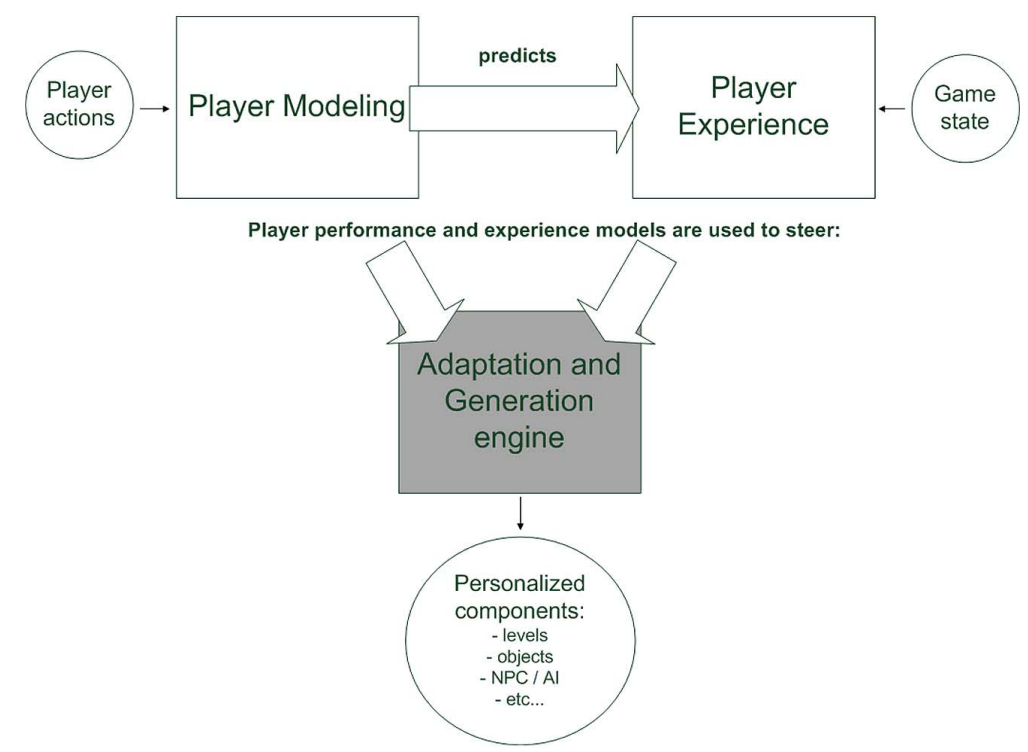
\includegraphics[width=0.75\textwidth]{ch2ddaarch}
	\caption{Přehled principů architektury adaptivních her. \cite{16Survey} }
	\label{fig:ch2ddaarch}
\end{figure}

V \cite{SwPatterns} se zabývali modelem DDA z pohledu návrhových vzorů objektového programování. Abstraktní model je znázorněn na obr. \ref{fig:ch2ddapatterns}. Senzory sbírají důležitá herní data, dle kterých se bude dále rozhodovat. Návrhový vzor Observer je připojen k Senzorům a v případě, že zaznamená zatelnou změnu v systému, vytvoří událost, trigger. Jednotlivé události jsou spojeny s akcemi a dohromady spolu tvoří pravidla uložená v databázi. V případě, že se spustí trigger spojený s akcí v některém z pravidel, rozhodne se v provedení této akce, což má na starost řadič, který má za úkol provést požadovanou změnu do stavu hry.

\begin{figure}
  \centering
  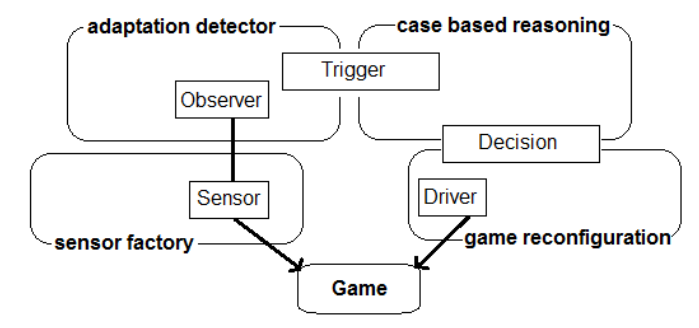
\includegraphics[width=0.75\textwidth]{ch2ddapatterns}
	\caption{Návrhové vzory DDA \cite{SwPatterns} }
	\label{fig:ch2ddapatterns}
\end{figure}

Dále se podíváme na jednotlivé návrhové vzory detailněji.

\subsection{Sensor factory}

Senzory jsou objekty, které pravidelně čtou herní data\footnote{Senzory nemusí zaznamenávat pouze herní data. Mohou zaznamenávat i prostředí uživatele např. pomocí Kinectu, nebo snímat aktuální tep hráče.} a upozorňují na změny zbytek DDA systému. Schéma návrhového vzoru znázorňuje obr. \ref{fig:ch2senzorfactory}. Senzor je abstraktní třídou, která zahrnuje periodické sbírání dat a upozorňující mechanismus. Konkrétní senzory z této třídy dědí a musí přepisovat abstraktní metodu refreshValue(), která zaznamenává konkrétní proměnnou systému. Třída SenzorFactory je zodpovědná za vytváření jednotlivých senzorů a je implementací návrhového vzoru factory. Továrna na senzory vyžaduje název senzoru a objekt, který má monitorovat. Vytvořené senzory si ukládá do registru. V případě, že uživatel zažádá o senzor, který už někdo vytvořil, dostane referenci na tento senzor. V opačném případě zkontroluje v ResourceManageru, jestli vytvořením nového senzoru se poruší některá z omezení zdrojů a pokud ne, senzor vytvoří.

\begin{figure}
  \centering
  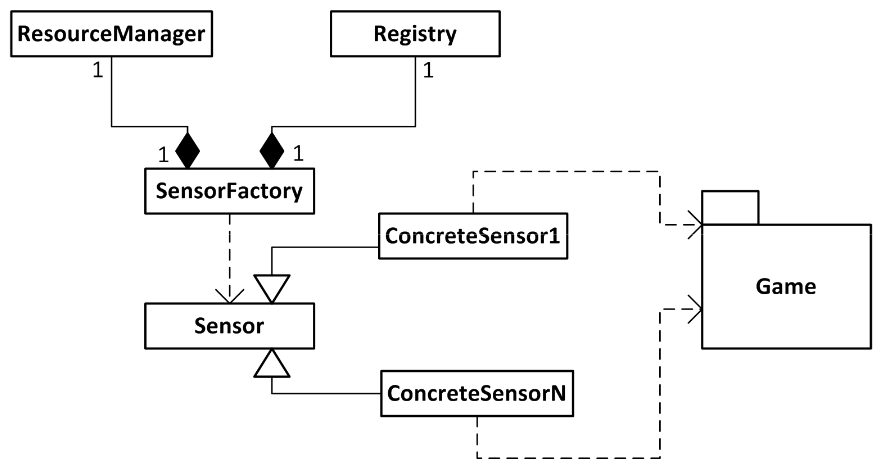
\includegraphics[width=0.5\textwidth]{ch2senzorfactory}
	\caption{Návrhový vzor sensor factory. \cite{SwPatterns} }
	\label{fig:ch2senzorfactory}
\end{figure}

\subsection{Adaptation detector}

Hrubá data získaná senzory se musí dále zpracovat. Tyto data získává AdaptationDetector pomocí observeru z návrhového vzoru senzor-observer. Na tomto místě se rozhoduje, jestli senzory již zaznamenaly dostatečnou změnu systému. Nedostatečnou změnou může být vystřelení jednoho náboje z plně nabitého revolveru. Naopak vystřílení půlky zásobníku může být významné. O významnost změny se stará TreshholdAnalyzer s Tresholdem. Treshold uchovává parametr hranice a její typ. (menší rovno, větší apod.) V případě dosažení prahu TresholdAnalyzer dá vědět AdaptationDetectoru, který vytvoří trigger, spouštěč. Trigger s sebou může nést další dodatečné informace jako je např. množství přeživších nepřátel. Viz obr. \ref{fig:ch2adaptationdesing}.

\begin{figure}
  \centering
  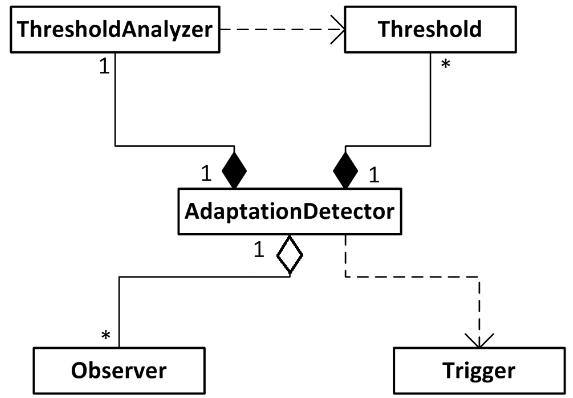
\includegraphics[width=0.5\textwidth]{ch2adaptationdesing}
	\caption{Návrhový vzor sensor factory. \cite{SwPatterns} }
	\label{fig:ch2adaptationdesing}
\end{figure}

\subsection{Case based reasoning}

Trigger spustí rozhodování na základě případů. Tento návrhový vzor(obr. \ref{fig:ch2casebase}) se použije, jestliže je možné vyvažování obtížnosti definovat konečným množstvím případů. InferenceEngine obsahuje dvě datové struktury: TriggerPool a FixedRules. Fixed rules obsahují pravidla, která jsou úzce spojená s konkrétní hrou. Pravidlo je kombinací triggeru a akce/rozhodnutí. TriggerPool funguje jako fronta událostí. Do fronty se řadí spuštěné triggery a jsou obsluhovány od nejstaršího. InferenceEngine vždy odebere jeden trigger z poolu, najde ho v databázi FixedRules pravidel a s ním nalezne vhodné rozhodnutí, které se má dále provést.

\begin{figure}
  \centering
  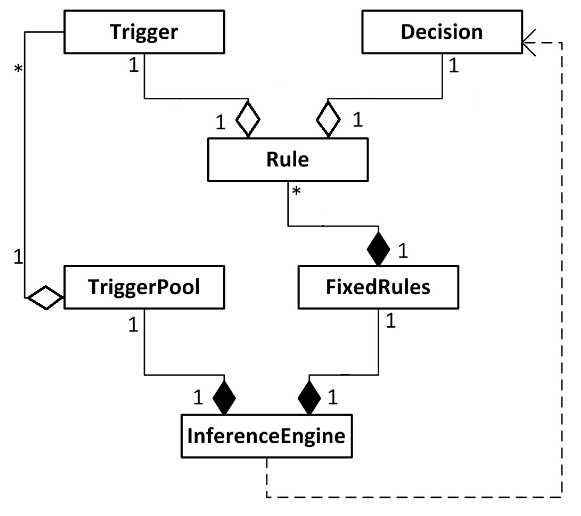
\includegraphics[width=0.5\textwidth]{ch2casebase}
	\caption{Návrhový vzor Case based reasoning. \cite{SwPatterns} }
	\label{fig:ch2casebase}
\end{figure}

\subsection{Game reconfiguration}

Posledním krokem je provedení požadované změny v herním světě. Návrhový vzor Game reconfiguration(obr. \ref{fig:ch2gamereco}) v sobě obsahuje jiný návrhový vzor, adapter. AdaptationDriver dostane ke zpracování rozhodnutí z InferenceEnginu. AdaptationDriver provede rozhodnutí za pomoci Driveru. Driver mění objekty, jež implementují rozhraní State, přes které zjišťuje aktuální stav objektu. S provedením jeho změny čeká dokud se nestane objekt neaktivním.

\begin{figure}
  \centering
  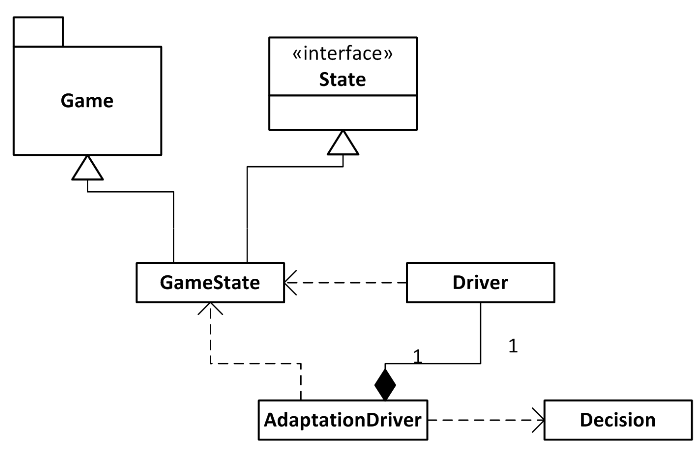
\includegraphics[width=0.5\textwidth]{ch2gamereco}
	\caption{Návrhový vzor Game reconfiguration. \cite{SwPatterns} }
	\label{fig:ch2gamereco}
\end{figure}

\section{Flow}

V předchozích kapitolách jsem zmínil hlavní směr většiny DDA programů. Vyrovnávat obtížnost vzhledem k dovednostem uživatele aplikací. S tímto souvisí pojem Flow.

\subsection{Definice}

Flow (tok) je stav mysli, kdy je osoba v průběhu provozování činnosti naprosto soustředěná, pociťuje nadšení, úspěch. „Flow je stav vědomí, kdy je člověk plně zaujatý svou činností. Nezabývá se jinými stimuly z okolí ani svými myšlenkami nebo pocity. Je naprosto soustředěný na prováděnou činnost. Dosahuje většinou, na své poměry, nadprůměrných výkonů, ale přitom mu to nepůsobí výraznou námahu. Je to harmonický zážitek, kdy tělo a mysl spolu bez námahy spolupracují. Tento stav je většinou spojen s pocity energie, radosti, harmonie a seberealizace.“ \cite{FlowCZ} S pojmem Flow prvně přišel zástupce pozitivní psychologie Mihaly Csikszentmihalyi ve své práci Flow: The psychology of optimal experience, česky vydané pod názvem O štěstí a smyslu života.

Požadovaný stav lze charakterizovat z pohledu dovedností člověka a náročnosti prováděné činnosti. Dosáhneme ho, jestliže provádíme úkol náročností odpovídající našim schopnostem. Viz obr. \ref{fig:ch2flow}. 

Jestliže se člověk seznamuje s novou činností, začíná v levém dolním rohu flow grafu. V tu chvíli nemá žádné dovednosti a pravděpodobně se začíná učit provádět činnost od jednoduchých částí po složitější. V knize \cite{OptimalFun} uvádí Csikszentmihalyi jako příklad takové činnosti hraní tenisu a vysvětluje to na obr. \ref{fig:ch2flow}. Alex začíná hrát tenis, a tedy se nachází ve fázi označené $A_1$. Alex v této chvíli neumí vůbec hrát tenis a začíná s tréninkem trefování se do míčku. Není to příliš obtížné, ale Alex si to užívá, protože náročnost tohoto úkolu přesně odpovídá jeho schopnostem.

\begin{figure}
  \centering
  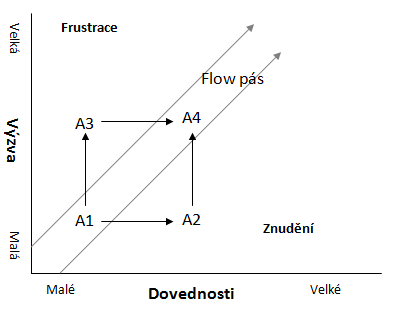
\includegraphics[width=0.5\textwidth]{ch2flow}
	\caption{Příklad pohybu jedince ve flow grafu. \cite{OptimalFun} }
	\label{fig:ch2flow}
\end{figure}

V této chvíli se Alex pohybuje v tzv flow pásu. Na stejném místě v diagramu nemůže zůstat Alex věčně. Jak danou činnost procvičuje, stává se v ní čím dál lepší, přestává ho to bavit, dostává se do nudy znázorněné v grafu $A_2$. V opačném případě se může stát, že potká zkušeného hráče. Hra proti němu je mnohem náročnějším úkolem a převyšuje Alexovy schopnosti. Alex se v takovém případě dostává do stavu úzkosti a stresu $A_3$.

V obou zmíněných příkladech se Alex nachází mimo flow pás a bude se snažit do něj opět dostat. V horším případě hru vzdá a další stav $A_4$ již v grafu nebude. V případě, že je ve stavu $A_2$, je dalším logickým krokem začít obtížnější úkol, vytyčit si nový cíl odpovídající jeho schopnostem. Ve stavu stresu $A_3$ má Alex jedinou možnost, zlepšit své dovednosti, aby se opět vrátil do flow pásu. Teoreticky může ubrat na výzvě, náročnosti úkolu, ale jak je jednou člověk vystaven takové výzvě, je pro něj těžké ji ignorovat a vzdát se jí. \cite{OptimalFun}

Dle Csikszentmihalyi se flow skládá z devíti elementů. \cite{FlowEng} Ne všechny jsou nutně potřebné k dosažení stavu flow.

\begin{enumerate}
	\item Jasné cíle
	\item Jednoznačná zpětná vazba
	\item Vyrovnanost náročnosti úkolů a schopností
	\item Splynutí činnosti a vědomí
	\item Koncentrace
	\item Žádné obavy z neúspěchu
	\item Pocit kontroly
	\item Změna vnímání času
	\item Vnitřní motivace
\end{enumerate}

Rozepisování jednotlivých bodů není záměrem této práce. Bližší informace lze nalézt např. na \cite{FlowEng}, \cite{FlowCZ}, nebo v originální knize \cite{OptimalFun}.

\subsection{Flow ve hrách}

Nás bude více zajímat napojení flow na vývoj počítačových her. Jenova Chen ve své diplomové práci Flow in Games\cite{thesisflow} vybral několik flow komponent, které označil za hlavní při návrhu hry. Dle Chena musí hra obsahovat následující tři elementy, aby hráč dosáhl stavu flow.

\begin{enumerate}
	\item Předpokladem je, že hra sama o sobě je pro hráče odměňující. Hráč sám o sobě chce hru hrát.
	\item Hra nabízí správnou náročnost úkolů vzhledem k hráčovým schopnostem, což mu umožňuje více se do hry ponořit.
	\item Hráč potřebuje cítit kontrolu nad prováděnou činností.
\end{enumerate}

Jsou-li splněny všechny tři body, hráč může ztratit pojem o čase a zcela se do hry ponořit.

Vraťme se znovu ke flow diagramu \ref{fig:ch2flow}. Dle příkladu s Alexem a jeho učením se tenisu by se mohlo zdát, že pro každého je ideální udržovat zcela vyrovnanou hodnotu schopností a náročnosti úkolů a udržovat uživatele v úzkém flow pásu, jak znázorňuje obr. \ref{fig:ch2flowzone1}.

\begin{figure}
  \centering
  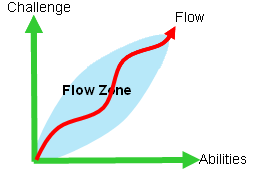
\includegraphics[width=0.5\textwidth]{ch2flowzone1}
	\caption{Obecně je vhodné hráče udržovat ve flow zóně. \cite{thesisflow} }
	\label{fig:ch2flowzone1}
\end{figure}	

Bohužel takový flow diagram nebere v úvahu individualitu hráče. Existují hráči, kteří mají rádi větší výzvy než jsou v tu chvíli schopni zvládnout, lze je nazvat hardcore hráči. Naopak existují příležitostní hráči, kteří netouží po velkých výzvách a nejraději se budou pohybovat lehce pod flow zónou. Těchto specifik si všímá např. práce \cite{RiskTakers}. Ideální průběh hry pro příležitostné/začínající hráče, běžné hráče a hardcore hráče znázorňuje graf na obr. \ref{fig:ch2flowzone2}. Mnohé práce tato specifika opomíjejí a často je jejich cílem upravit obtížnost hry, aby byl vyrovnaný počet hráčových výher a proher a už neberou v potaz, že někteří hráči přestanou hrát, když budou z poloviny pokusů prohrávat.

\begin{figure}
  \centering
  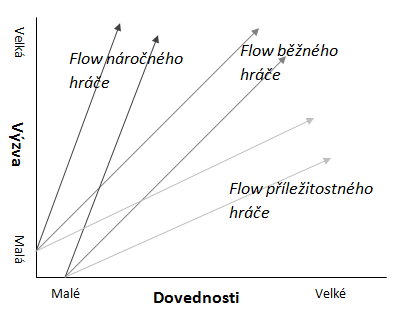
\includegraphics[width=0.5\textwidth]{ch2flowzone2}
	\caption{Flow zóna a specifika pro příležitostné a hardcore hráče. \cite{thesisflow} }
	\label{fig:ch2flowzone2}
\end{figure}	

\subsection{Pozitivní a negativní odezva}

\section{Definice zábavy a jak ji měřit} \label{sec:defzab}



